\documentclass[_main.tex]{subfiles}
 
\begin{document}

\section*{Introduction}

Quantitative models of infectious disease transmission are important in planning public health strategies for disease control \cite{Ross1915,Smith2012}.  By analysing variation in the genome sequence of parasites sampled over space and time, it is in principle possible to derive information about the recent history and dynamics of host to host transmission that cannot readily be obtained by other means.

Current methods for inference of transmission dynamics from genomic surveillance data are mostly based on an approach known as phylodynamics \cite{Grenfell2004,Volz2013}, whose starting point is to construct a phylogenetic tree representing the genetic relationship between isolates.  This approach works well for viruses such as SARS-CoV-2 in epidemic scenarios where recombination can essentially be ignored.  However it runs into problems when there is frequent recombination combined with \textit{superinfection}, meaning that a host acquires infection from multiple independent sources.  This is the case for many parasitic microorganisms including some viruses and bacteria as well as sexually-reproducing eukaryotic parasites.

The fundamental problem is that a superinfected host carries a mixture of parasite genotypes with different ancestral histories, which may then be \textit{cotransmitted} to other hosts.  Recombination within genetically mixed infections causes different regions of the genome to have different genealogies (figure \ref{fig:superinfection1}).  This presents an extremely complex problem for genealogical inference  \cite{Speidel2019, Kelleher2019} and conventional phylodynamic approaches do not work in this situation, because the parasite population cannot be represented by a single phylogenetic tree.

\begin{figure}[h!]
\centering
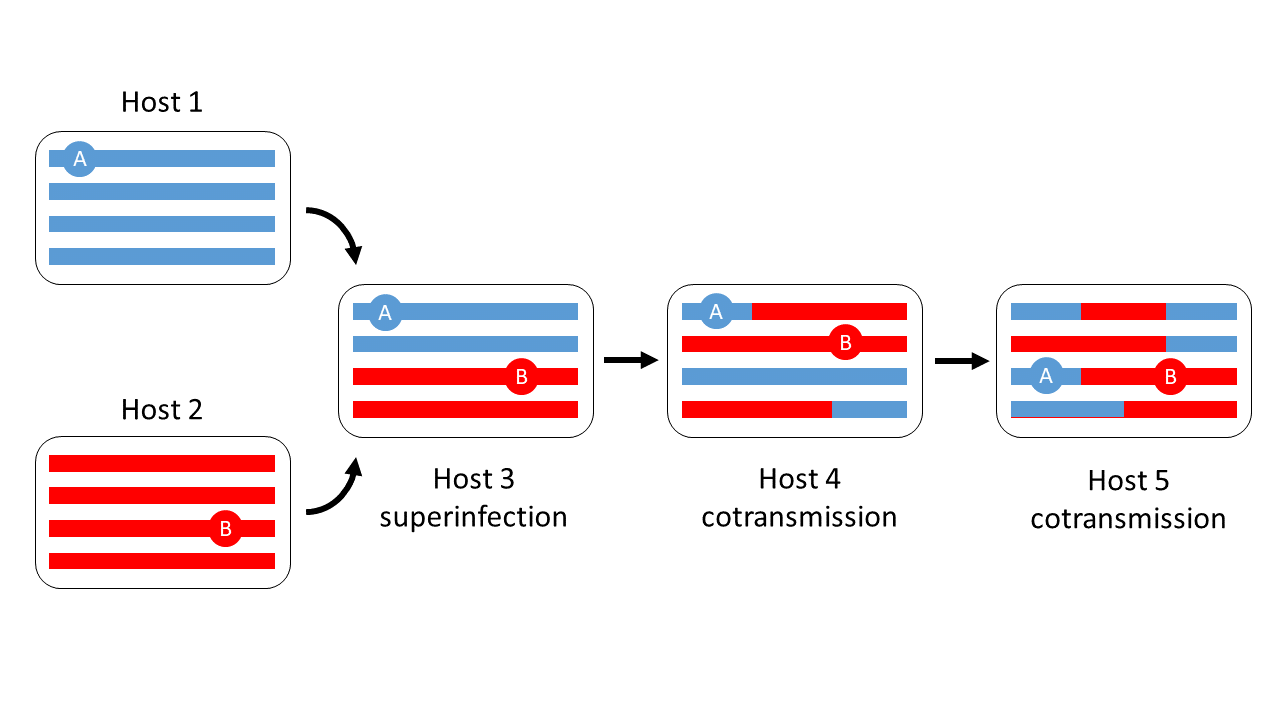
\includegraphics[width=12cm]{221102_superinfection.png}
\caption{\textbf{Superinfection leads to cotransmission and recombination of distinct lineages.}  Coloured bars represent parasite genomes within a host.  Here we imagine that hosts 1 and 2 each carry a clonal population of parasites, and that the two clonal populations can be differentiated by genotyping, represented by blue and red respectively.  Host 3 is superinfected and carries a mixture of the two genotypes.  The two genotypes recombine when this mixture is cotransmitted from host 3 to host 4, and there is further recombination when the mixture is cotransmitted from host 4 to host 5.  The circles marked A and B represent two different loci in a parasite genome carried by host 5: locus A is inherited from host 1 whereas locus B is inherited from host 2.  Thus it is not possible to represent this parasite population by a single phlyogenetic tree - because the red/blue recombinant genomes cannot be mapped onto a single position on the tree.}
\label{fig:superinfection1}
\end{figure}

\paragraph{Malaria as an example.} 

Malaria provides an interesting paradigm for exploring this problem because people living in some parts of the world are bitten by malaria-infected mosquitoes many times per year \cite{Smith2005,WHO2022}.  In these areas of high transmission, it is common for an infected person to carry a mixture of parasite genotypes, either due to superinfection (because they have been bitten by multiple mosquitoes each carrying parasites from a different source) or due to cotransmission (because they have been bitten by a mosquito that is carrying parasites with mixed genotypes due to superinfection of a previous host) \cite{Nkhoma2020}.  The malaria parasites undergo sexual reproduction in the mosquito, allowing cotransmitted genomes to recombine.

Thus malaria infections have a broad spectrum of genetic complexity that reflects the local transmission dynamics.  In regions of low transmission intensity, where superinfection is rare, most infections are essentially clonal.  In regions of high transmission intensity, many infections comprise a mixture of parasites with distinct genotypes, and these can have complex pedigree structures due to repeated cycles of cotransmission and sexual recombination \cite{Nkhoma2020}. 

\paragraph{Modelling a parasite population with superinfection and recombination.} 

One approach to this problem is to build an epidemiological model of malaria transmission coupled to a separate model that simulates the process of genetic variation \cite{Daniels2015,Watson2020,Hendry2021}.  This allows many biological and epidemiological features to be incorporated into the model, but it tends to be computationally laborious and requires considerable guesswork about parameter values.  

Here we describe an alternative approach to modelling the relationship between transmission dynamics and population genetics, based on an idealised transmission graph that takes account of superinfection and cotransmission.  We show how this naturally yields a Markov process for coalescent simulation of a recombining parasite population as well as providing a theoretical framework for estimation of transmission parameters from empirical genetic observations.  

This paper is theoretical but is illustrated with empirical data relating to the human malaria parasite \textit{Plasmodium falciparum}.  \textit{P. falciparum} parasites are single-celled haploid organisms that are transmitted from host to host by a mosquito vector.  The parasites reproduce prolifically within the host and vector.  Their mode of reproduction is asexual, except at a specific point of the transmission cycle within the mosquito vector, when sexual forms mate to produce recombinant offspring that are transmitted to the next human host (see glossary figure \ref{fig:one_generation}).

For clarity, in describing our model we shall use the terms parasite, host and vector to refer specifically to malaria.  By \textit{parasite} we mean a haploid individual of the species \textit{P. falciparum}; a \textit{host} is a person that is carrying parasites and is capable transmitting them to others; and a \textit{vector} is a mosquito that transmits parasites from one host to another.  However this does not mean that the model is applicable only to malaria, and with suitable modification most of the underlying concepts could equally be applied to other parasites and recombining populations in general. 

A \hyperref[supp_glossary]{glossary of terminology} is included before the Methods section.  Analyses shown in figures and tables use the open source Python package \texttt{coalestr}.  Worked examples and tutorials on using \texttt{coalestr} are available at \href{https://d-kwiat.github.io/gtg}{\texttt{d-kwiat.github.io/gtg}}. 

\end{document}